\section{Validation du design}
Lors de cette section, sera décrite la procédure de vérification des caractéristiques du projet ainsi la validation de celui-ci.
\subsection{Liste de matériel}
{
	\begin{enumerate}
		\item Oscilloscope Tektronix RTB2004 ES.SLO2.05.01.16
		\item USB Logic Analyzer, 8-Canaux, 24MHz
		\item USB TO TLL HW-597
		\item Carte Localisation-Sous-Marine V0.0
	\end{enumerate}
}

\subsection{Contrôle des alimentations}
{
	En premier lieu, une vérification des tensions d'alimentation permet de valider un aspect critique et fondamentale de la carte.
	\subsubsection{Méthodologie}
	\paragraph{Mesure du 3.3V :} Alimentation de la carte par une connections brève entre les pins du connecteur du bouton \textbf{P15}. Mesure sur le testpoint \textit{V\_regOUT5} voir figure \ref{fig:sch3}.
	\begin{figure}[h]
		\centering
		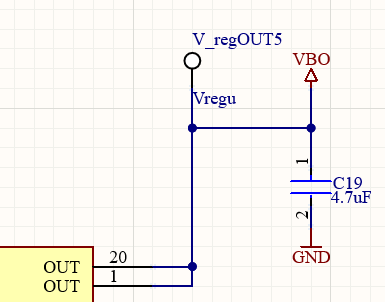
\includegraphics[width=0.3\linewidth]{Figures/DEV_MEAS/Sch3.3V}
		\caption{Testpoint mesure 3.3V}
		\label{fig:sch3}
	\end{figure}
	
	\paragraph{Mesure du 5V :} Pour mesurer le 5V, il faut ponter par une résistance $0\Omega$ la résistance R50, ainsi que activer la Pin RC5 / EN\_5V. Ensuite la mesure a été prise sur le connecteur P16, pin-3 :
	\begin{figure}[h]
		\centering
		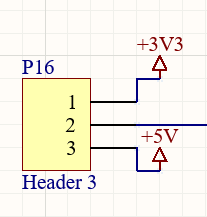
\includegraphics[width=0.2\linewidth]{Figures/DEV_MEAS/Sch5V}
		\caption{Schéma de mesure 5V}
		\label{fig:sch5v}
	\end{figure}

	\clearpage
	
	\subsubsection{Mesures}
	
	\begin{figure}
	\begin{subfigure}{.5\textwidth}
		\centering
		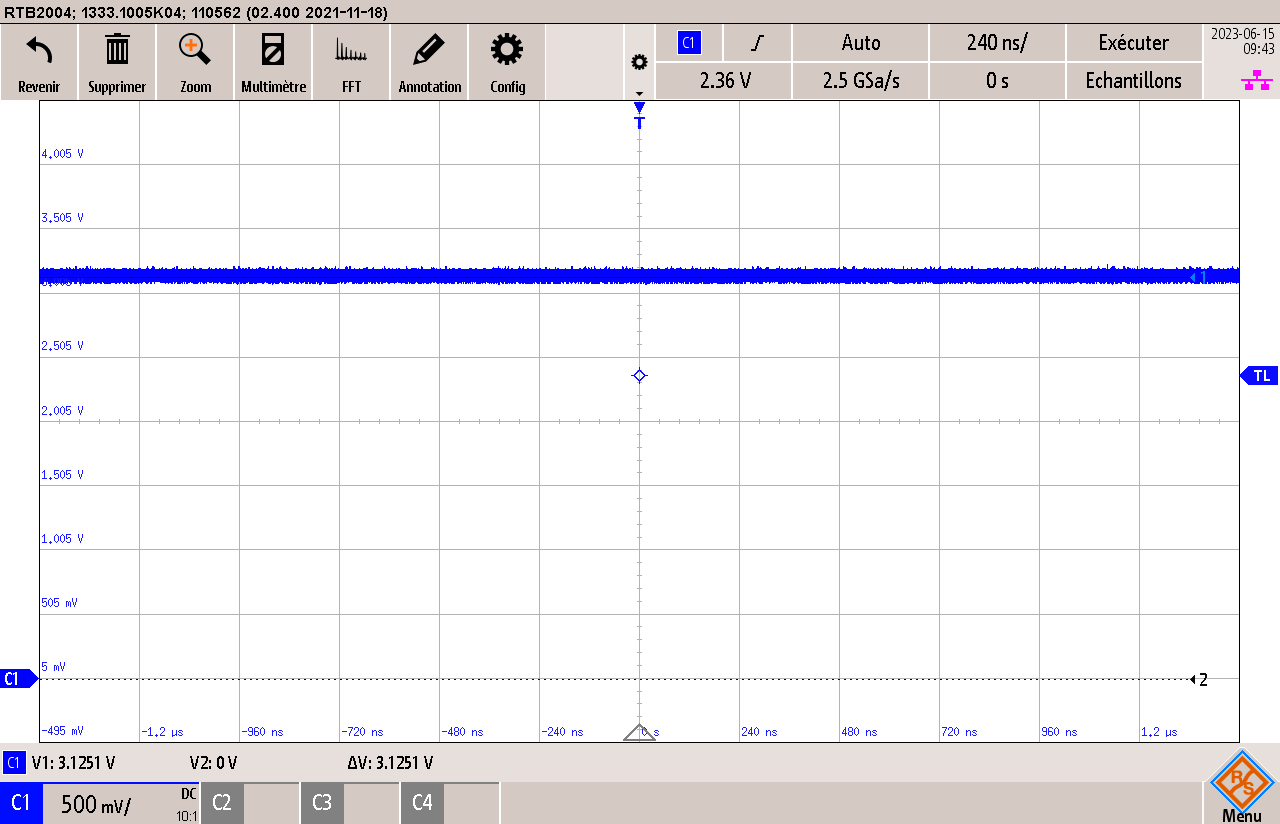
\includegraphics[width=\textwidth]{Mesures/Tension3.3V}
		\caption{Mesure 3.3V}
		\label{fig:Mes3.3V}
	\end{subfigure}
	\begin{subfigure}{.5\textwidth}
		\centering
		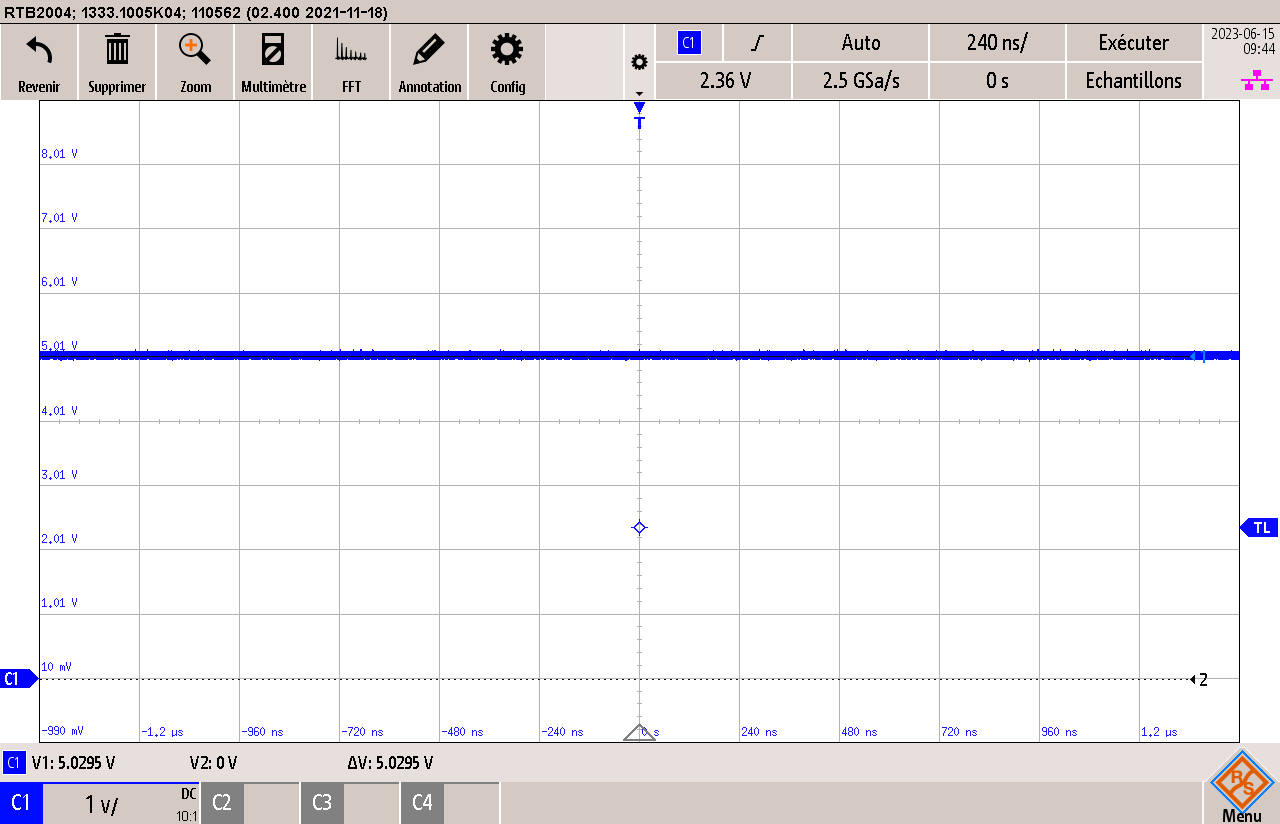
\includegraphics[width=\textwidth]{Mesures/Tension5V}
		\caption{Mesure 5V}
		\label{fig:Mes5V}
	\end{subfigure}
	\caption{Mesures des tensions d'alimentations}
	\label{fig:Mesure3.3et5V}
	\end{figure}
	
	\paragraph{Analyse :} On peut constater que les valeurs des tensions respective sur les figures \ref{fig:Mes3.3V} et \ref{fig:Mes5V}, sont proches. La tension d'alimentation du microcontrôleur est 3.125V ce qui peut être expliqué par une chute de la tension de la batterie LI-ION qui a besoin d'être chargée. La tension 3.3V oscille un peu, sachant qu'il s'agit de l'alimentation de l'entièreté de la carte et que des signaux rapides sont générés.
	
}

\subsection{Communication UART}
{
	\subsubsection{Méthodologie}
	
	\subsubsection{Mesures}

}

\subsection{Communication SPI, carte SD}
{
	\subsubsection{Méthodologie}
	
	\subsubsection{Mesures}

}

\section{Caractéristiques du produit finis}
